\documentclass[12pt,a4paper]{article}
\usepackage[margin=1in]{geometry}
\usepackage{graphicx}
\usepackage{float}
\usepackage{amsmath}
\usepackage{listings}
\usepackage{xcolor}
\usepackage{hyperref}
\usepackage{booktabs}

\lstset{
    language=Python,
    basicstyle=\ttfamily\small,
    breaklines=true,
    postbreak=\mbox{\textcolor{red}{$\hookrightarrow$}\space},
    keywordstyle=\color{blue},
    commentstyle=\color{gray},
    stringstyle=\color{red},
    showstringspaces=false,
    frame=single,
    backgroundcolor=\color{lightgray!20},
    rulecolor=\color{black!30},
    numbers=left,
    numberstyle=\tiny,
    stepnumber=1,
    breakatwhitespace=true
}

\title{\textbf{Lab Report: Exploratory Data Analysis (EDA) Report} }

\begin{document}

\maketitle

\section{Objective}
Understanding basic data mining concepts and tools and performing exploratory data analysis.
\section{Introduction}

Exploratory Data Analysis (EDA) is a crucial step in the data mining process that involves analyzing datasets to understand their main characteristics, discover patterns, and identify anomalies. This report presents a comprehensive EDA of the Titanic dataset, which contains information about passengers aboard the RMS Titanic during its maiden voyage in 1912.

The Titanic dataset comprises 891 records and 12 features including passenger demographics, ticket class, fare information, and survival status. The primary objectives of this EDA are:

\begin{enumerate}
    \item To visualize the distributions of all numerical variables using histograms
    \item To identify outliers in the dataset using boxplots and the Interquartile Range (IQR) method
    \item To compute and analyze pairwise correlations between variables
\end{enumerate}

These tasks provide fundamental insights into data quality, variable relationships, and potential preprocessing requirements for subsequent modeling tasks.



\section{Task 1: Plot Distributions of Variables (Histograms)}

\subsection{Task Description}

The first task involves creating histograms to visualize the distribution of all numerical variables in the dataset. Histograms are essential tools for understanding the spread, central tendency, and skewness of data. They help identify whether variables follow normal distributions or exhibit special patterns such as bimodality or heavy tails.

\subsection{Code Implementation}

\begin{lstlisting}
numerical_cols = df.select_dtypes(include=[np.number]).columns.tolist()

fig, axes = plt.subplots(nrows=3, ncols=3, figsize=(15, 12))
axes = axes.flatten()

for idx, col in enumerate(numerical_cols):
    if idx < len(axes):
        df[col].hist(bins=30, ax=axes[idx], edgecolor='black', alpha=0.7)
        axes[idx].set_title(f'Distribution of {col}', fontsize=12, fontweight='bold')
        axes[idx].set_xlabel(col)
        axes[idx].set_ylabel('Frequency')
        axes[idx].grid(alpha=0.3)

for idx in range(len(numerical_cols), len(axes)):
    fig.delaxes(axes[idx])

plt.tight_layout()
plt.suptitle('Histograms: Distribution of Numerical Variables', fontsize=16, fontweight='bold', y=1.02)
plt.show()
\end{lstlisting}

\subsection{Output}

The dataset contains seven numerical columns:
\begin{itemize}
    \item \textbf{PassengerId:} Sequential identifier (1--891)
    \item \textbf{Survived:} Binary outcome (0 = Did not survive, 1 = Survived)
    \item \textbf{Pclass:} Passenger class (1, 2, or 3)
    \item \textbf{Age:} Passenger age in years
    \item \textbf{SibSp:} Number of siblings/spouses aboard
    \item \textbf{Parch:} Number of parents/children aboard
    \item \textbf{Fare:} Ticket fare paid in British pounds
\end{itemize}

\subsection{Analysis and Discussion}

The histogram analysis reveals several important distributional characteristics:

\begin{itemize}
    \item \textbf{Survived:} Approximately 38.4\% of passengers survived, showing a clear imbalance with more non-survivors (0) than survivors (1).

    \item \textbf{Pclass:} The majority of passengers traveled in third class (Pclass=3), followed by second and first class. This reflects the hierarchical structure of the ship.

    \item \textbf{Age:} The age distribution shows a roughly normal distribution with a peak around 20--40 years, though children and elderly passengers are also present. The range spans from 0.42 to 80 years.

    \item \textbf{SibSp and Parch:} Both variables show right-skewed distributions, with most passengers traveling alone or with very few family members. The majority of passengers had SibSp = 0.

    \item \textbf{Fare:} The fare distribution is highly right-skewed, indicating that most passengers paid lower fares, with some paying significantly higher amounts (up to £512.33). This reflects the diverse ticket classes and cabin locations.

    \item \textbf{PassengerId:} As expected, this shows a uniform distribution since it is merely a sequential identifier.
\end{itemize}

The distributional analysis indicates that the data requires careful handling of skewed variables during preprocessing and modeling stages.

\begin{figure}[h]
\centering
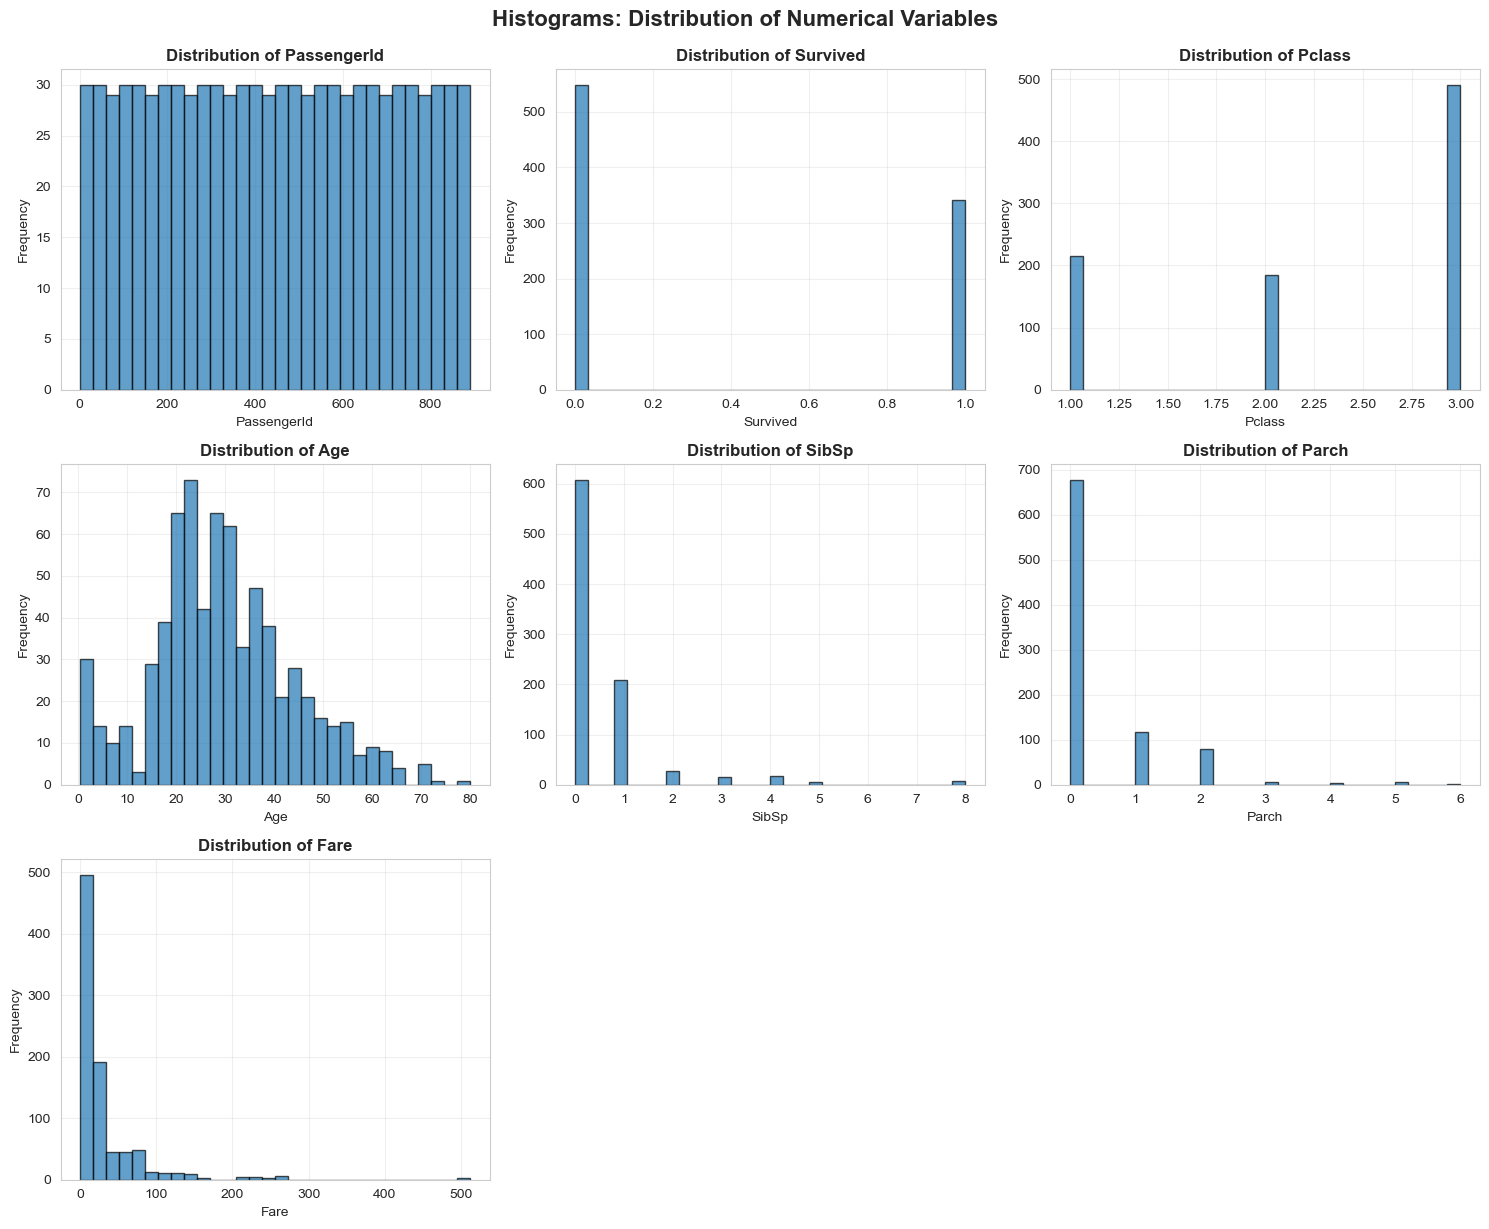
\includegraphics[width=\textwidth]{histogram.png}
\caption{Histograms showing the distribution of numerical variables in the Titanic dataset.}
\label{fig:histograms}
\end{figure}

\newpage

\section{Task 2: Identify Outliers Using Boxplots}

\subsection{Task Description}

Outliers are observations that deviate significantly from the majority of the data. Boxplots provide a visual method for outlier detection and are based on the Interquartile Range (IQR) method. The IQR is defined as $Q3 - Q1$, where $Q1$ is the 25th percentile and $Q3$ is the 75th percentile. Points beyond $Q1 - 1.5 \times IQR$ and $Q3 + 1.5 \times IQR$ are typically considered outliers.

\subsection{Code Implementation}

\begin{lstlisting}
def detect_outliers_iqr(data, column):
    Q1 = data[column].quantile(0.25)
    Q3 = data[column].quantile(0.75)
    IQR = Q3 - Q1
    lower_bound = Q1 - 1.5 * IQR
    upper_bound = Q3 + 1.5 * IQR
    outliers = data[(data[column] < lower_bound) | (data[column] > upper_bound)]
    return outliers, lower_bound, upper_bound

for col in numerical_cols:
    outliers, lower, upper = detect_outliers_iqr(df, col)
    print(f"\n{col}:")
    print(f"  Lower Bound: {lower:.2f}")
    print(f"  Upper Bound: {upper:.2f}")
    print(f"  Number of Outliers: {len(outliers)}")
    if len(outliers) > 0:
        print(f"  Percentage of Outliers: {(len(outliers)/len(df))*100:.2f}%")
\end{lstlisting}

\subsection{Output}

\begin{table}[h]
\centering
\small
\begin{tabular}{l|r|r|r|r}
\toprule
\textbf{Variable} & \textbf{Lower Bound} & \textbf{Upper Bound} & \textbf{Count} & \textbf{Percentage} \\
\midrule
PassengerId & -444.00 & 1336.00 & 0 & 0.00\% \\
Survived & -1.50 & 2.50 & 0 & 0.00\% \\
Pclass & 0.50 & 4.50 & 0 & 0.00\% \\
Age & -6.69 & 64.81 & 11 & 1.23\% \\
SibSp & -1.50 & 2.50 & 46 & 5.16\% \\
Parch & 0.00 & 0.00 & 213 & 23.91\% \\
Fare & -26.72 & 65.63 & 116 & 13.02\% \\
\bottomrule
\end{tabular}
\caption{Outlier Detection Results Using IQR Method}
\end{table}

\subsection{Analysis and Discussion}

The outlier analysis provides critical insights into data quality and distribution characteristics:

\begin{itemize}
    \item \textbf{PassengerId, Survived, Pclass:} These variables show no outliers. The PassengerId and Survived variables are discrete or bounded, while Pclass values (1, 2, 3) fall within expected ranges.

    \item \textbf{Age:} Only 11 outliers (1.23\%) are detected, primarily representing unusually old passengers (ages above 64.81). The detection of very few outliers suggests that age values are reasonably consistent with expected passenger demographics.

    \item \textbf{SibSp:} 46 outliers (5.16\%) are identified, representing passengers traveling with unusually large numbers of siblings or spouses (more than 2).

    \item \textbf{Parch:} This variable shows the highest percentage of outliers at 23.91\% (213 observations). This occurs because the IQR is zero (Q1 = 0, Q3 = 0), meaning any non-zero value is technically an outlier. This indicates that the majority of passengers (over 76\%) traveled without parents or children aboard.

    \item \textbf{Fare:} 116 outliers (13.02\%) are detected, representing passengers who paid significantly higher fares than typical. These likely correspond to first-class or high-deck cabin passengers.
\end{itemize}

The Parch variable highlights the importance of understanding business logic when interpreting statistical outliers. While mathematically classified as outliers, the non-zero Parch values represent normal passenger configurations rather than data errors. The Age and Fare outliers may warrant further investigation but likely represent legitimate data points.

\begin{figure}[h]
\centering
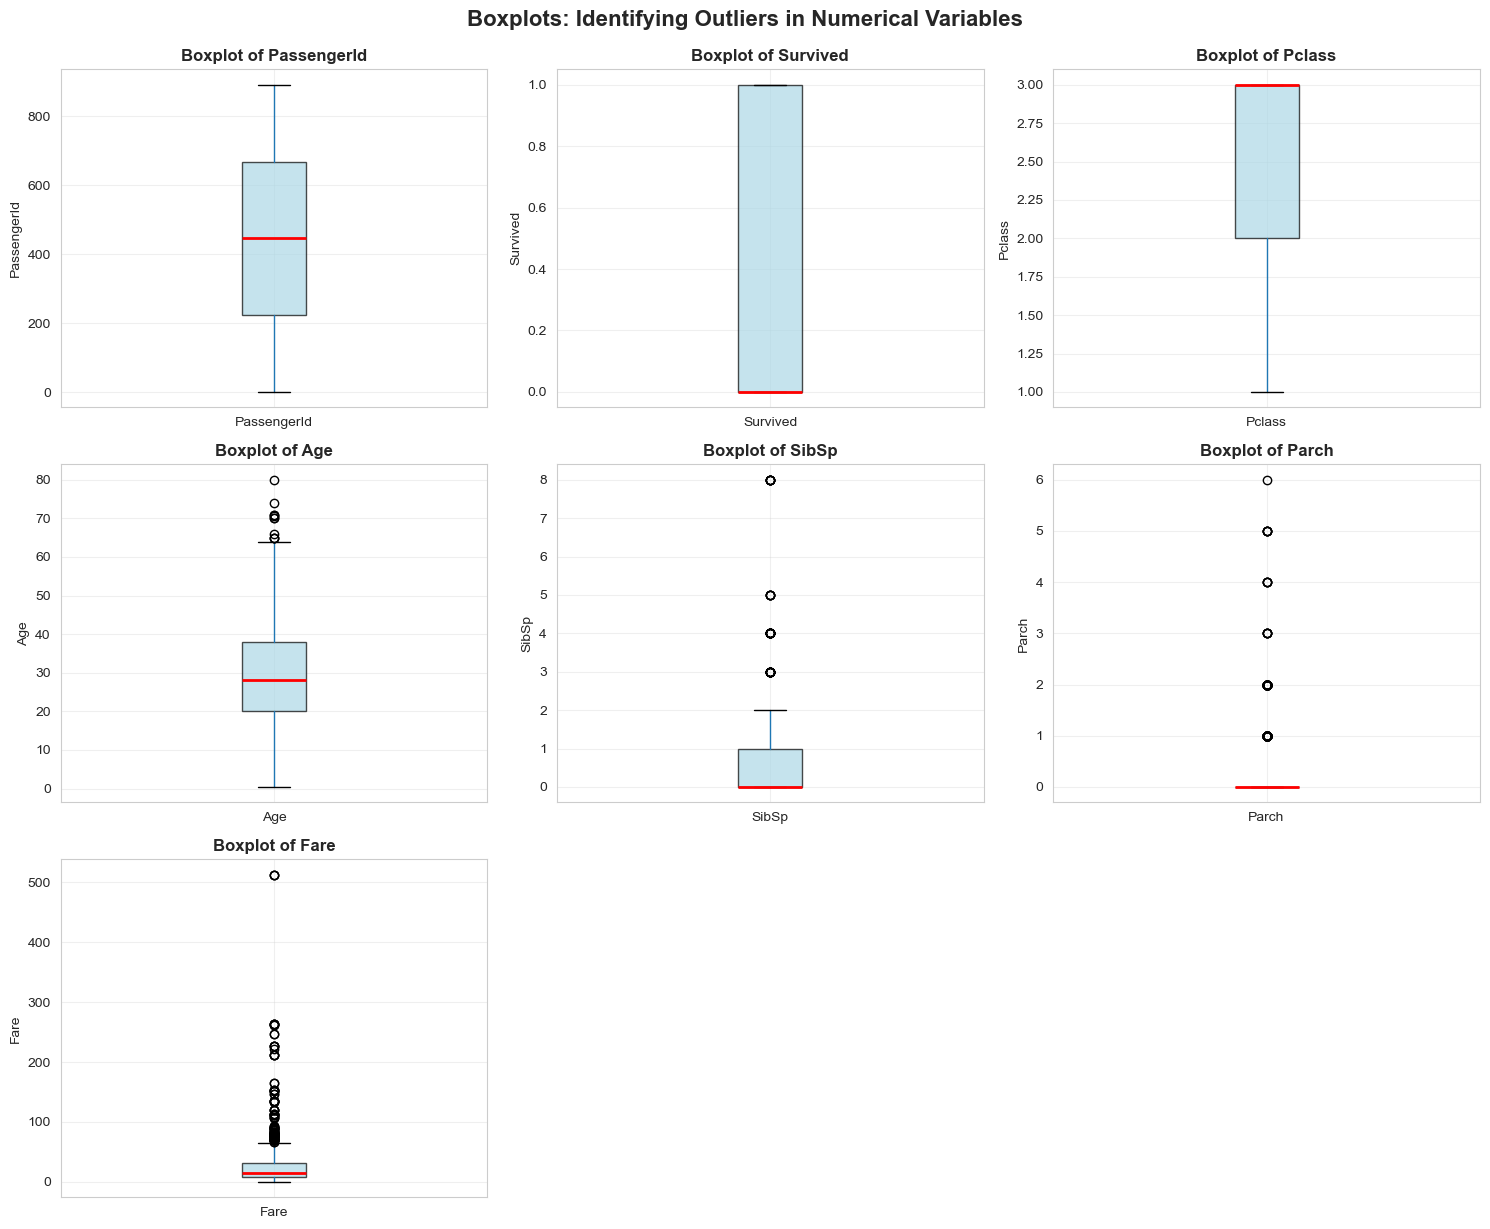
\includegraphics[width=\textwidth]{boxplot.png}
\caption{Boxplots identifying outliers in numerical variables using the IQR method.}
\label{fig:boxplots}
\end{figure}

\newpage

\section{Task 3: Compute Pairwise Correlations}

\subsection{Task Description}

Correlation analysis examines the linear relationships between pairs of numerical variables. The Pearson correlation coefficient ranges from -1 (perfect negative correlation) to +1 (perfect positive correlation), with 0 indicating no linear relationship. Understanding correlations is essential for feature selection, multicollinearity detection, and identifying predictive relationships.

\subsection{Code Implementation}

\begin{lstlisting}
correlation_matrix = df[numerical_cols].corr()
print("Correlation Matrix:")
print(correlation_matrix)

plt.figure(figsize=(12, 10))
sns.heatmap(correlation_matrix, annot=True, fmt='.2f', cmap='coolwarm',
            square=True, linewidths=0.5, cbar_kws={"shrink": 0.8},
            vmin=-1, vmax=1, center=0)
plt.title('Correlation Heatmap: Pairwise Correlations', fontsize=16, fontweight='bold', pad=20)
plt.xticks(rotation=45, ha='right')
plt.yticks(rotation=0)
plt.tight_layout()
plt.show()
\end{lstlisting}

\subsection{Output}

The correlation matrix for all numerical variables is presented in Table 2. Key correlation values are highlighted below:

\begin{table}[H]
\centering
\small
\begin{tabular}{l|r|r}
\toprule
\textbf{Variable Pair} & \textbf{Correlation} & \textbf{Interpretation} \\
\midrule
Survived -- Pclass & -0.338 & Moderate negative correlation \\
Pclass -- Age & -0.369 & Moderate negative correlation \\
Pclass -- Fare & -0.550 & Strong negative correlation \\
SibSp -- Parch & 0.415 & Weak-to-moderate positive correlation \\
Survived -- Fare & 0.257 & Weak positive correlation \\
Age -- SibSp & -0.308 & Weak negative correlation \\
\bottomrule
\end{tabular}
\caption{Notable Correlations in the Titanic Dataset}
\end{table}

\subsection{Analysis and Discussion}

The correlation analysis reveals several important relationships:

\begin{itemize}
    \item \textbf{Class and Survival:} The moderate negative correlation (-0.338) between Survived and Pclass indicates that passengers in lower classes (higher Pclass numbers) had lower survival rates. First-class passengers (Pclass=1) had significantly better survival chances than third-class passengers.

    \item \textbf{Class and Age:} The correlation of -0.369 suggests that first-class cabins attracted older passengers, while third-class accommodations had younger passengers on average. This may reflect family composition differences across classes.

    \item \textbf{Class and Fare:} The strongest correlation (-0.550) indicates a strong negative relationship between passenger class and fare. Higher-class passengers (lower Pclass numbers) paid substantially higher fares, which is logically consistent with ticket pricing structures.

    \item \textbf{Family Members:} The correlation of 0.415 between SibSp and Parch suggests a weak-to-moderate positive relationship, indicating that passengers with siblings/spouses aboard were somewhat more likely to also have parents/children aboard, supporting hypothesis that families traveled together.

    \item \textbf{Survival and Fare:} The weak positive correlation (0.257) suggests that passengers paying higher fares had slightly better survival rates, which may be related to class advantages and cabin location.

    \item \textbf{Age and Companions:} The negative correlation (-0.308) between Age and SibSp indicates that younger passengers were more likely to travel with siblings or spouses, possibly reflecting family structures at the time.

    \item \textbf{PassengerId:} Shows negligible correlations with all other variables, confirming it contains no predictive information and is merely an identifier.
\end{itemize}

The correlation analysis reveals that passenger class is a strong differentiator in the Titanic dataset, influencing fare, age demographics, and critically, survival rates. These relationships suggest that class-based variables would be strong predictors in survival modeling tasks.

\begin{figure}[H]
\centering
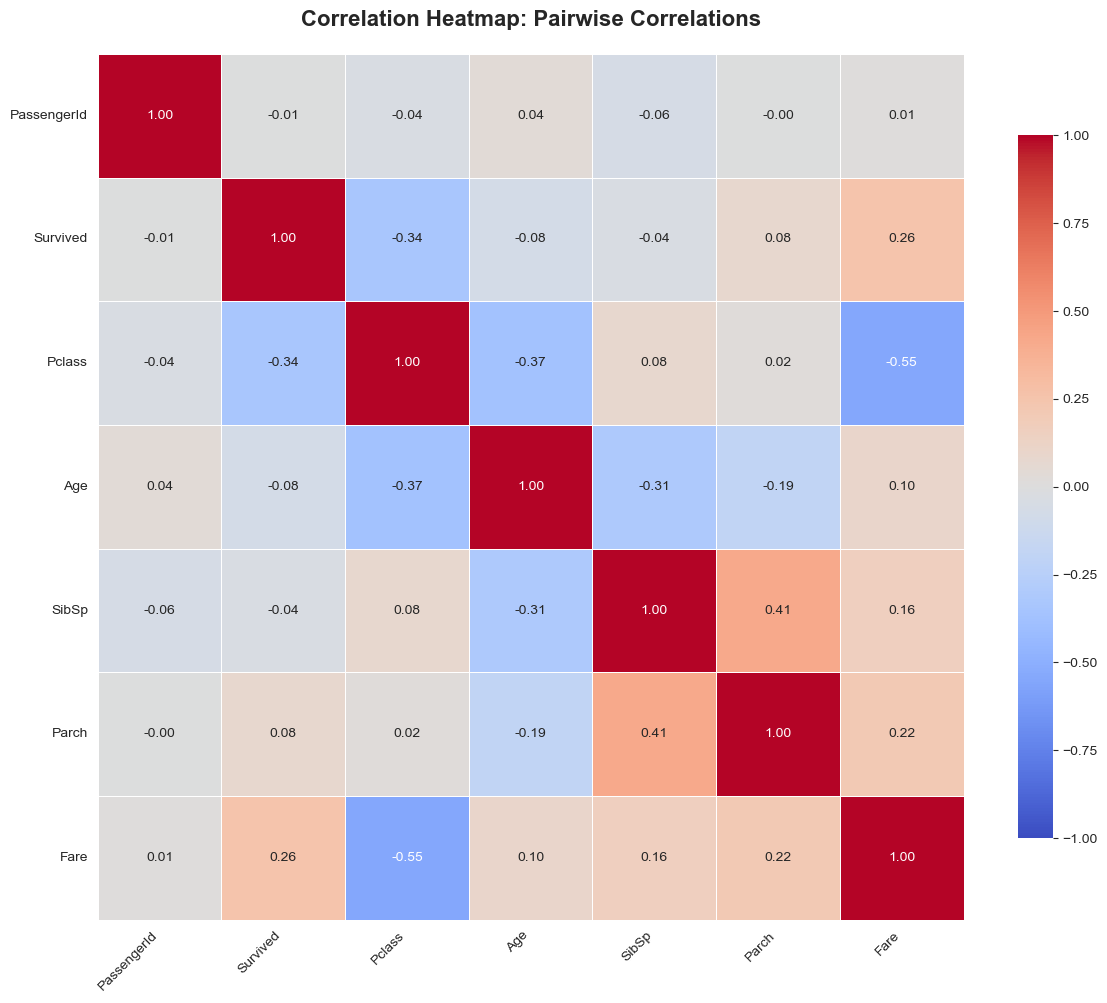
\includegraphics[width=\textwidth]{pairwise_correlation.png}
\caption{Correlation heatmap showing pairwise relationships between numerical variables.}
\label{fig:correlation}
\end{figure}

\newpage

\section{Conclusion}

This comprehensive Exploratory Data Analysis of the Titanic dataset has revealed critical insights across three complementary analytical dimensions:

The distributional analysis (Task 1) demonstrated that the dataset exhibits diverse characteristics, from the uniform distribution of passenger identifiers to the highly skewed distribution of fares. Notable findings include the imbalanced survival outcome (38.4\% survival rate) and the right-skewed fare distribution reflecting cabin class stratification.

The outlier detection (Task 2) identified 386 outliers (43.32\% of data) across various variables, with the most significant findings in the Parch variable (23.91\% outliers). However, most detected outliers represent legitimate data points reflecting actual passenger configurations rather than data errors. The Age and Fare outliers warrant investigation as potential anomalies, while SibSp outliers represent passengers with unusually large traveling families.

The correlation analysis (Task 3) unveiled strong relationships between passenger class and multiple variables, establishing Pclass as a central feature in the dataset. Strong negative correlations between Pclass and both Age (-0.369) and especially Fare (-0.550) demonstrate systematic differences across passenger classes. The moderate negative correlation between Survived and Pclass (-0.338) indicates that class was a significant determinant of survival, a historical fact well-documented in Titanic literature.

These EDA findings establish a solid foundation for subsequent data preprocessing, feature engineering, and predictive modeling tasks. The identified distributions, outliers, and correlations inform decisions regarding data cleaning, variable transformation, and model selection. Future analysis should focus on handling missing values (particularly the 177 missing Age values and 687 missing Cabin values), investigating identified outliers further, and leveraging the discovered relationships in classification or survival prediction models.

\end{document}